\documentclass[conference]{IEEEtran}
\IEEEoverridecommandlockouts

\usepackage{cite}
\usepackage{amsmath,amssymb,amsfonts}
\usepackage{graphicx}
\usepackage{textcomp}
\usepackage{xcolor}
\usepackage{booktabs}
\usepackage{url}
\urlstyle{same}
\usepackage{tikz}
\usetikzlibrary{arrows.meta,positioning,shapes.geometric,calc}
\usepackage{fancyhdr}
\pagestyle{fancy}
\fancyhf{}
\fancyfoot[C]{\thepage}
\renewcommand{\headrulewidth}{0pt}
\definecolor{psiicolor}{RGB}{70,130,180}
\definecolor{psicolor}{RGB}{46,158,107}
\definecolor{leafgreen}{RGB}{46,158,107}

\def\BibTeX{{\rm B\kern-.05em{\sc i\kern-.025em b}\kern-.08em
    T\kern-.1667em\lower.7ex\hbox{E}\kern-.125emX}}

\begin{document}

\title{Photosynthesis -- Mechanisms, Efficiency, and Relevance for Renewable Energy Systems}

\author{\IEEEauthorblockN{Eliah Graf}
\IEEEauthorblockA{\textit{Faculty of Electrical Engineering} \\
\textit{Technische Hochschule Ulm}\\
Ulm, Germany \\
grafel01@thu.de}
}

\maketitle

\begin{abstract}
Photosynthesis is the biological process by which plants and other organisms convert sunlight, water, and carbon dioxide into chemical energy stored as biomass. Although photosynthesis and photovoltaic (PV) technology share the same energy source -- sunlight -- they differ fundamentally in their conversion mechanisms, efficiencies, and outputs. This paper examines the core mechanisms of photosynthesis, including the light-dependent reactions governed by Photosystem I and II and the light-independent Calvin cycle, with a focus on energy conversion from an engineering perspective. Efficiency limits and the key loss mechanisms that reduce solar-to-biomass conversion to roughly 1\% in field conditions and up to 4\% under optimal controlled conditions are analyzed and contrasted with commercial silicon PV modules achieving 18--20\%. Finally, the emerging field of artificial photosynthesis is discussed as a complementary technology for producing solar fuels and renewable chemical feedstocks.
\end{abstract}

\begin{IEEEkeywords}
photosynthesis, photovoltaics, solar energy, energy conversion efficiency, artificial photosynthesis, renewable energy, Z-scheme, Calvin cycle
\end{IEEEkeywords}

%% ---------------------------------------------------------------
\section{Introduction}

The global transition toward renewable energy systems demands a broad understanding of natural and engineered solar energy conversion processes. Photosynthesis -- the mechanism by which plants, algae, and cyanobacteria harness sunlight -- represents the most widespread solar energy converter on Earth. It has sustained nearly all life on the planet for billions of years and currently underpins biomass energy, an important pillar of the renewable energy mix.

From the perspective of electrical engineering and energy systems, photosynthesis is of interest not only as a biological phenomenon but as an energy conversion system that can be analyzed, benchmarked, and potentially replicated. Both photosynthesis and photovoltaic (PV) technology convert electromagnetic radiation into a storable form of energy, yet their underlying principles, efficiencies, and outputs differ substantially.

This paper is structured as follows. Section~II provides an overview of the two stages of photosynthesis. Section~III examines the energy conversion mechanisms in detail, focusing on Photosystem I (PSI) and Photosystem II (PSII). Section~IV analyzes the theoretical maximum efficiency and the main loss mechanisms. Section~V compares photosynthesis to PV technology. Section~VI discusses artificial photosynthesis as a pathway toward solar fuels. Section~VII concludes the paper.

%% ---------------------------------------------------------------
\section{Fundamentals of Photosynthesis}

Photosynthesis takes place in two sequential stages: the light-dependent reactions and the light-independent reactions (the Calvin cycle). Together, they convert solar photons, water, and carbon dioxide into glucose and oxygen according to the overall reaction:

\begin{equation}
6\,\text{CO}_2 + 6\,\text{H}_2\text{O} + \text{light} \;\longrightarrow\; \text{C}_6\text{H}_{12}\text{O}_6 + 6\,\text{O}_2
\end{equation}

Fig.~\ref{fig:overview} shows the two-stage structure of photosynthesis and the flow of energy carriers between them.

\begin{figure}[t]
\centering
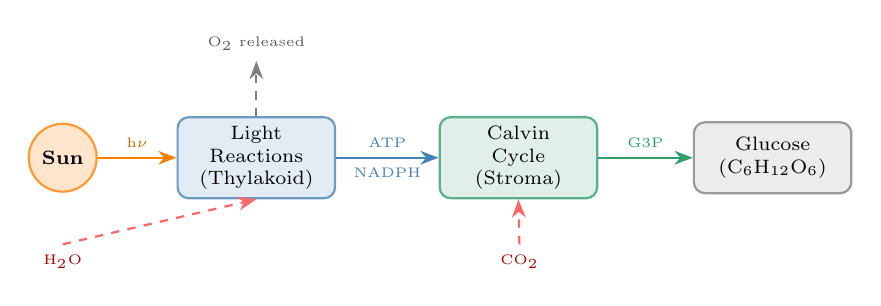
\begin{tikzpicture}[
  box/.style={rectangle, rounded corners=4pt, draw=#1!80, fill=#1!15, thick,
              minimum width=2.0cm, minimum height=0.9cm, align=center, font=\scriptsize},
  arr/.style={-{Stealth}, thick, #1},
  lbl/.style={font=\tiny, #1}
]
  % Sunlight input
  \node[circle, draw=orange!80, fill=orange!20, thick,
        minimum size=0.85cm, font=\scriptsize\bfseries] (sun) at (0,0) {Sun};

  % Light reactions box
  \node[box=psiicolor, right=1.0cm of sun] (lr) {Light\\Reactions\\(Thylakoid)};

  % Calvin cycle box
  \node[box=psicolor, right=1.3cm of lr] (cc) {Calvin\\Cycle\\(Stroma)};

  % Outputs box
  \node[box=gray, right=1.2cm of cc] (out) {Glucose\\(C$_6$H$_{12}$O$_6$)};

  % Arrows
  \draw[arr=orange] (sun) -- node[above, lbl=orange!80!black] {h$\nu$} (lr);
  \draw[arr=psiicolor] (lr) -- node[above, lbl=psiicolor] {ATP} node[below, lbl=psiicolor] {NADPH} (cc);
  \draw[arr=psicolor] (cc) -- node[above, lbl=psicolor] {G3P} (out);

  % Inputs below
  \draw[arr=red!60, dashed] (0.0,-1.1) node[below, lbl=red!70!black] {H$_2$O} -- (lr.south);
  \draw[arr=red!60, dashed] (5.8,-1.1) node[below, lbl=red!70!black] {CO$_2$} -- (cc.south);

  % Byproduct O2
  \draw[arr=gray, dashed] (lr.north) -- ++(0,0.7) node[above, lbl=gray!70!black] {O$_2$ released};

\end{tikzpicture}
\caption{Overview of the two-stage photosynthesis process. Light reactions in the thylakoid membrane convert sunlight, water, and ADP/NADP$^+$ into ATP, NADPH, and O$_2$. The Calvin cycle uses these energy carriers to fix CO$_2$ into glucose.}
\label{fig:overview}
\end{figure}

\subsection{Light-Dependent Reactions}
The light-dependent reactions occur in the thylakoid membranes of chloroplasts. Their primary outputs are adenosine triphosphate (ATP) and nicotinamide adenine dinucleotide phosphate (NADPH), which serve as energy carriers for the subsequent Calvin cycle. Oxygen is released as a byproduct of water splitting \cite{libretexts_general}.

\subsection{Calvin Cycle}
The Calvin cycle (also called the light-independent reactions) takes place in the stroma of the chloroplast. Using the ATP and NADPH generated in the light-dependent stage, carbon dioxide is fixed by the enzyme RuBisCO and reduced to form glyceraldehyde-3-phosphate (G3P), a precursor to glucose and other organic molecules. The Calvin cycle does not directly require light but depends entirely on the products of the light reactions \cite{libretexts_openStax}.

%% ---------------------------------------------------------------
\section{Energy Conversion Mechanisms}

\subsection{The Z-Scheme}
The electron flow through the light-dependent reactions is described by the \textit{Z-scheme}, named for its characteristic shape when electron energy is plotted against the reaction sequence. Electrons are boosted twice by light absorption -- once in PSII and once in PSI -- allowing them to reach a sufficiently high energy level to reduce NADP\textsuperscript{+} to NADPH \cite{bioninja}. Fig.~\ref{fig:zscheme} illustrates this energy diagram.

\begin{figure*}[t]
\centering
\begin{tikzpicture}[scale=0.82, font=\scriptsize]
  % Y-axis label
  \draw[->] (-0.2,0) -- (-0.2,5.8) node[left, rotate=90, anchor=south, xshift=-10pt] {\scriptsize Redox Potential (more negative $\uparrow$)};

  % --- PSII side ---
  \draw[thick, psiicolor] (0.2,0.5) -- (1.8,0.5);
  \node[right, font=\scriptsize] at (1.8,0.5) {P680 (ground)};
  \draw[-{Stealth}, thick, orange] (1.0,0.5) -- (1.0,4.2) node[midway, left=2pt, font=\scriptsize] {h$\nu$ 680\,nm};
  \draw[thick, psiicolor] (0.2,4.2) -- (1.8,4.2);
  \node[right, font=\scriptsize] at (1.8,4.2) {P680*};

  % ETC chain
  \draw[-{Stealth}, dashed, gray] (1.8,4.2) -- (3.2,3.6);
  \draw[thick, gray!70] (2.8,3.6) -- (4.2,3.6);
  \node[right, font=\scriptsize] at (4.2,3.6) {Pheo/PQ};
  \draw[-{Stealth}, dashed, gray] (4.2,3.6) -- (5.4,3.0);
  \draw[thick, gray!70] (5.0,3.0) -- (6.4,3.0);
  \node[right, font=\scriptsize] at (6.4,3.0) {Cyt b6f};
  \draw[-{Stealth}, dashed, gray] (6.4,3.0) -- (7.6,2.6);
  \draw[thick, gray!70] (7.2,2.6) -- (8.4,2.6);
  \node[right, font=\scriptsize] at (8.4,2.6) {PC};

  % ATP label
  \node[orange!80!black, font=\scriptsize\bfseries] at (5.2,3.45) {ATP};

  % Water splitting
  \draw[-{Stealth}, thick, red!70!black] (1.0,0.05) -- (1.0,0.5);
  \node[below, red!70!black, font=\scriptsize] at (1.0,0.0) {H$_2$O $\to$ O$_2$ + e$^-$};

  % --- PSI side ---
  \draw[thick, psicolor] (8.0,2.6) -- (9.6,2.6);
  \node[right, font=\scriptsize] at (9.6,2.6) {P700 (ground)};
  \draw[-{Stealth}, thick, orange] (8.8,2.6) -- (8.8,5.4) node[midway, right=2pt, font=\scriptsize] {h$\nu$ 700\,nm};
  \draw[thick, psicolor] (8.0,5.4) -- (9.6,5.4);
  \node[right, font=\scriptsize] at (9.6,5.4) {P700*};

  % To Fd and NADPH
  \draw[-{Stealth}, dashed, gray] (9.6,5.4) -- (10.8,4.9);
  \draw[thick, gray!70] (10.4,4.9) -- (11.8,4.9);
  \node[right, font=\scriptsize] at (11.8,4.9) {Fd};
  \draw[-{Stealth}, dashed, leafgreen, very thick] (11.8,4.9) -- (12.8,4.4);
  \draw[thick, leafgreen] (12.4,4.4) -- (13.8,4.4);
  \node[right, font=\scriptsize\bfseries, leafgreen] at (13.8,4.4) {NADPH};

  % Labels
  \node[psiicolor, font=\scriptsize\bfseries] at (1.0,4.9) {PSII};
  \node[psicolor, font=\scriptsize\bfseries] at (8.8,5.9) {PSI};
\end{tikzpicture}
\caption{Simplified Z-scheme energy diagram. Electrons are excited twice by photon absorption (orange arrows), flow through the electron transport chain generating ATP, and ultimately reduce NADP$^+$ to NADPH. Water is oxidized at PSII to replenish electrons.}
\label{fig:zscheme}
\end{figure*}

\subsection{Photosystem II (PSII)}
PSII contains a reaction-center chlorophyll pair known as P680, which absorbs photons at a wavelength of approximately 680~nm. Upon light absorption, one electron is excited to a higher energy state and transferred to an electron acceptor, initiating the electron transport chain. The electron deficit in P680 is replenished by the oxidative splitting of water molecules (photolysis), which releases molecular oxygen and protons:

\begin{equation}
2\,\text{H}_2\text{O} \;\longrightarrow\; 4\,\text{H}^+ + 4\,e^- + \text{O}_2
\end{equation}

As electrons travel through the chain of protein complexes between PSII and PSI (plastoquinone, the cytochrome b6f complex, and plastocyanin), their energy is used to pump protons across the thylakoid membrane, building a proton gradient. This gradient drives ATP synthase, producing ATP from ADP and inorganic phosphate -- a mechanism directly analogous to the proton-motive force used in mitochondrial respiration \cite{slcc_etc}.

\subsection{Photosystem I (PSI)}
By the time electrons reach PSI, they have lost a significant portion of their initial energy during transport. PSI's reaction center, P700, absorbs photons at approximately 700~nm and provides a second energy boost to re-excite these electrons. The re-energized electrons are ultimately transferred via ferredoxin to NADP\textsuperscript{+} reductase, which catalyzes the reduction of NADP\textsuperscript{+} to NADPH \cite{libretexts_general, libretexts_openStax}:

\begin{equation}
\text{NADP}^+ + 2\,e^- + \text{H}^+ \;\longrightarrow\; \text{NADPH}
\end{equation}

In addition to linear electron flow, PSI can engage in cyclic electron flow, recycling electrons back to the cytochrome b6f complex to produce additional ATP without generating NADPH. This regulatory mechanism allows the cell to balance the ATP/NADPH ratio according to metabolic demand \cite{wikipedia_ldr}.

\subsection{Energy Summary}
The net result of the light-dependent reactions can be summarized as the conversion of photon energy into the chemical bond energy of ATP and NADPH. Four photons are required per electron pair extracted from water; since two electrons are needed to reduce one NADP\textsuperscript{+}, and the Calvin cycle consumes three ATP and two NADPH per CO\textsubscript{2} fixed, the total photon cost per molecule of CO\textsubscript{2} fixed is approximately eight photons \cite{ripe_pdf}.

%% ---------------------------------------------------------------
\section{Efficiency Analysis}

\subsection{Theoretical Maximum Efficiency}
The theoretical maximum efficiency of oxygenic photosynthesis under ideal assumptions is often quoted at approximately 13\% of total solar radiation \cite{academia_max}. When only photosynthetically active radiation (PAR, wavelengths 400--700~nm) is considered, the ceiling rises to roughly 9.4\% for C3 plants and approximately 10.8\% for C4 plants \cite{ripe_pdf}. More conservative estimates for real plants under standard conditions yield practical upper limits of about 4.6\% (C3) and 6\% (C4) \cite{academia_max, oamonitor}.

\subsection{Key Loss Mechanisms}
Real-world photosynthetic efficiency falls far below these theoretical limits due to a cascade of loss mechanisms:

\begin{itemize}
    \item \textbf{Spectral losses:} Plants can only use radiation in the PAR range. Infrared and ultraviolet radiation, which together constitute a substantial fraction of the solar spectrum, are not absorbed by chlorophyll and are therefore unavailable for photochemistry \cite{ripe_pdf}.
    
    \item \textbf{Reflection and transmission:} A fraction of incident PAR is reflected by the leaf surface or transmitted through the leaf without being absorbed \cite{repository_up}.
    
    \item \textbf{Thermodynamic losses in charge separation:} When a photon excites an electron in P680 or P700, only a portion of the photon energy is stored in the excited state; the remainder is lost as heat due to rapid internal conversion and vibrational relaxation \cite{repository_up}.
    
    \item \textbf{Electron transport chain losses:} As electrons flow downhill through the transport chain, a portion of their energy is dissipated as heat rather than being stored in the proton gradient. This represents an intrinsic thermodynamic cost of the system \cite{sciencedirect_losses}.
    
    \item \textbf{Photorespiration:} In C3 plants, the enzyme RuBisCO can mistakenly bind O\textsubscript{2} instead of CO\textsubscript{2} in a wasteful competing reaction. This process, called photorespiration, consumes ATP and NADPH without producing useful carbon compounds and can reduce net photosynthetic efficiency by 25\% or more under warm, high-oxygen conditions \cite{pmc_efficiency}.
    
    \item \textbf{Non-photochemical quenching (NPQ):} When light intensity exceeds the capacity of the Calvin cycle, excess absorbed energy is deliberately dissipated as heat or fluorescence to protect the photosynthetic machinery from oxidative damage. While essential for plant survival, NPQ reduces the fraction of absorbed light that contributes to photochemistry \cite{sciencedirect_losses, repository_up}.
    
    \item \textbf{Respiration and maintenance costs:} A portion of the fixed carbon is consumed by cellular respiration and other metabolic processes, reducing the net biomass accumulation available as an energy output \cite{ars_usda_pubs}.
\end{itemize}

The combined effect of these losses is that typical crop plants achieve a seasonal average solar-to-biomass efficiency of only about 1\%, even under favorable field conditions \cite{ars_usda_news}.

%% ---------------------------------------------------------------
\section{Comparison with Photovoltaic Technology}

Table~\ref{tab:efficiency} summarizes the efficiency values for photosynthesis and competing solar energy conversion technologies.

\begin{table}[t]
\caption{Solar Energy Conversion Efficiency Comparison}
\begin{center}
\setlength{\tabcolsep}{4pt}
\begin{tabular}{p{2.4cm}p{1.6cm}p{3.6cm}}
\toprule
\textbf{System} & \textbf{Efficiency} & \textbf{Notes} \\
\midrule
Crop photosynthesis & $\sim$1\% (annual) & Field-scale, solar-to-biomass \cite{ars_usda_news} \\[2pt]
C3 plants (optimal) & $\sim$3.5\% & Controlled conditions \cite{uni_osnabrueck} \\[2pt]
C4 plants (optimal) & $\sim$4.3\% & Controlled conditions \cite{uni_osnabrueck} \\[2pt]
Commercial Si PV & 18--20\% & Module efficiency \cite{uni_osnabrueck} \\[2pt]
PV + electrolysis & 10--12\% & Solar-to-hydrogen \cite{ars_usda_news} \\
\bottomrule
\end{tabular}
\label{tab:efficiency}
\end{center}
\end{table}

PV cells convert photons directly into electric current via the photovoltaic effect, bypassing the many biological conversion steps that introduce losses in photosynthesis. A silicon PV cell absorbs a broader portion of the solar spectrum, operates without the overhead of cellular maintenance, and does not engage in competing reactions analogous to photorespiration \cite{pubmed_comparison}. Fig.~\ref{fig:efficiency} illustrates the efficiency gap visually.

\begin{figure}[t]
\centering
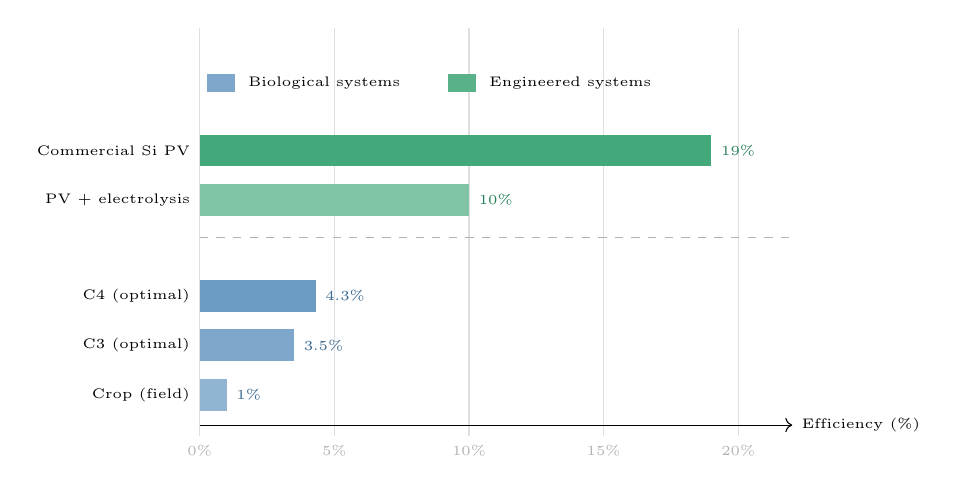
\begin{tikzpicture}[font=\scriptsize, scale=0.9]
  % Scale: 1cm = 1%,  max = 22%
  \def\scale{0.38}

  % Grid lines
  \foreach \x in {0,5,10,15,20} {
    \draw[gray!25, thin] (\x*\scale, -0.15) -- (\x*\scale, 5.6);
    \node[below, gray!60, font=\tiny] at (\x*\scale, -0.15) {\x\%};
  }

  % Bars (y positions from bottom)
  % Crop field 1.0%
  \fill[psiicolor!60] (0, 0.2)  rectangle (1.0*\scale,  0.65);
  \node[left, font=\tiny] at (0, 0.425) {Crop (field)};
  \node[right, font=\tiny, psiicolor!80!black] at (1.0*\scale, 0.425) {1\%};

  % C3 optimal 3.5%
  \fill[psiicolor!70] (0, 0.9)  rectangle (3.5*\scale,  1.35);
  \node[left, font=\tiny] at (0, 1.125) {C3 (optimal)};
  \node[right, font=\tiny, psiicolor!80!black] at (3.5*\scale, 1.125) {3.5\%};

  % C4 optimal 4.3%
  \fill[psiicolor!80] (0, 1.6)  rectangle (4.3*\scale,  2.05);
  \node[left, font=\tiny] at (0, 1.825) {C4 (optimal)};
  \node[right, font=\tiny, psiicolor!80!black] at (4.3*\scale, 1.825) {4.3\%};

  % PV + electrolysis 10%
  \fill[psicolor!60] (0, 2.95)  rectangle (10.0*\scale, 3.40);
  \node[left, font=\tiny] at (0, 3.175) {PV + electrolysis};
  \node[right, font=\tiny, psicolor!80!black] at (10.0*\scale, 3.175) {10\%};

  % Si PV 19%
  \fill[psicolor!90] (0, 3.65)  rectangle (19.0*\scale, 4.10);
  \node[left, font=\tiny] at (0, 3.875) {Commercial Si PV};
  \node[right, font=\tiny, psicolor!80!black] at (19.0*\scale, 3.875) {19\%};

  % Separator line between bio and PV
  \draw[dashed, gray!60, thin] (0, 2.65) -- (22*\scale, 2.65);
  \node[right, gray!70, font=\tiny] at (22*\scale, 2.65) {};

  % X axis
  \draw[->] (0,0) -- (22*\scale, 0) node[right, font=\tiny] {Efficiency (\%)};

  % Legend
  \fill[psiicolor!70] (0.1, 4.7) rectangle (0.5, 4.95);
  \node[right, font=\tiny] at (0.55, 4.825) {Biological systems};
  \fill[psicolor!80] (3.5, 4.7) rectangle (3.9, 4.95);
  \node[right, font=\tiny] at (3.95, 4.825) {Engineered systems};

\end{tikzpicture}
\caption{Solar energy conversion efficiency comparison. Biological systems (bottom group) achieve 1--4\%, while commercial silicon PV reaches $\sim$19\%. PV-driven electrolysis for H$_2$ production achieves $\sim$10\%.}
\label{fig:efficiency}
\end{figure}

However, a direct comparison requires acknowledging fundamental differences in outputs. PV produces electricity -- a high-quality, immediately usable energy form -- while photosynthesis produces biomass, a chemical energy carrier that can be stored, transported, and used as a feedstock for materials and fuels. PV-driven electrolysis (splitting water using PV-generated electricity) achieves approximately 10--12\% annual solar-to-hydrogen efficiency under realistic conditions, still significantly higher than natural photosynthesis, but at considerably higher infrastructure cost \cite{ars_usda_news, ars_usda_mag}.

The two systems are therefore best understood as complementary rather than competing: PV is superior for direct electricity generation per unit area, while photosynthesis offers self-replication, self-repair, and the direct synthesis of complex organic molecules -- capabilities that no current engineered system can replicate economically at scale \cite{pubmed_comparison}.

%% ---------------------------------------------------------------
\section{Artificial Photosynthesis}

\subsection{Concept and Motivation}
Artificial photosynthesis aims to replicate the core function of natural photosynthesis in engineered systems: using sunlight, water, and CO\textsubscript{2} to produce chemical fuels and feedstocks, without the biological overhead. The primary products of interest are hydrogen (via water splitting) and carbon-based fuels such as methanol or formic acid (via CO\textsubscript{2} reduction) \cite{satw_outlook, pmc_artificial}.

\subsection{Current State of Research}
Research in artificial photosynthesis spans several approaches, including photoelectrochemical (PEC) cells, molecular catalysts, photocatalytic suspensions, and semi-artificial systems that incorporate isolated biological components such as enzymes or reaction center proteins into synthetic frameworks. Recent work has explored materials including perovskites, quantum dots, two-dimensional materials, and metal-organic frameworks as light absorbers and catalysts \cite{sciencedirect_topic, altenergy_mag}.

Despite significant progress, the field remains predominantly at the laboratory and prototype stage. The key technical challenges are low solar-to-fuel efficiency, poor long-term stability of catalysts and photoabsorbers, slow reaction kinetics for multi-electron processes such as water oxidation, and high manufacturing costs for scalable systems \cite{pubmed_artificial, pmc_artificial}.

\subsection{Relevance for Energy Systems}
Artificial photosynthesis is strategically relevant for sectors that are difficult to electrify directly, including aviation, shipping, long-haul transport, and industrial chemistry (e.g., ammonia synthesis). In these applications, energy-dense liquid or gaseous fuels are more practical than batteries or direct electricity, and artificial photosynthesis offers a route to producing these fuels from sunlight in a carbon-neutral cycle \cite{pubs_aip, pubmed_comparison}.

In the near term, the most realistic pathway is likely the integration of PV-generated electricity with electrochemical synthesis, effectively decoupling the light-capture and catalytic steps. Longer-term, fully integrated photoelectrochemical devices that mimic the spatial organization of the chloroplast -- combining light absorption, charge separation, and catalysis in a single compact unit -- represent the ultimate engineering goal \cite{pmc_artificial, satw_outlook}.

%% ---------------------------------------------------------------
\section{Conclusion}

Photosynthesis is a sophisticated, multi-stage solar energy conversion system that has been optimized by evolution for biological survival rather than maximum energy yield. Its core mechanisms -- the Z-scheme electron transport through PSII and PSI, proton-gradient-driven ATP synthesis, and CO\textsubscript{2} fixation in the Calvin cycle -- provide an elegant framework for understanding biological solar energy conversion from an engineering perspective.

When benchmarked against photovoltaic technology, natural photosynthesis is substantially less efficient: typical field efficiencies of 1\% compare unfavorably with commercial silicon PV modules at 18--20\%. The gap arises from spectral limitations, thermodynamic losses, photorespiration, and the metabolic overhead of maintaining a living system.

Nevertheless, photosynthesis offers unique capabilities -- self-repair, self-replication, and direct production of complex organic molecules -- that make it irreplaceable in the current energy landscape. Artificial photosynthesis seeks to bridge the gap between biology and engineering, with the goal of producing renewable fuels from sunlight at efficiencies and costs that complement, rather than compete with, established PV and wind technologies. For the future of integrated renewable energy systems, both natural and artificial photosynthesis will play important roles alongside conventional solar electricity generation.

%% ---------------------------------------------------------------
\section*{Acknowledgment}
The author thanks Prof. Thomas Walter and the Seminar Erneuerbare Energien SS2026 at Technische Hochschule Ulm for the opportunity to explore this topic.

%% ---------------------------------------------------------------
\section*{Disclosure of AI Usage}
This paper was produced with the assistance of generative artificial intelligence tools. Perplexity AI (Deep Research) was used for literature search and source identification. Claude (Anthropic, claude-sonnet-4-6) was used to support paper structuring, drafting, and \LaTeX{} typesetting. All sources were identified and provided by the author; factual content was verified against the cited references. The final paper reflects the intellectual work and judgment of the author.

%% ---------------------------------------------------------------
\begin{thebibliography}{00}

\bibitem{libretexts_general}
LibreTexts Biology, ``The Light-Dependent Reactions of Photosynthesis,'' \textit{General Biology (Boundless)}, [Online]. Available: \url{https://bio.libretexts.org/Bookshelves/Introductory\_and\_General\_Biology/General\_Biology\_(Boundless)/08:\_Photosynthesis/8.06}

\bibitem{libretexts_openStax}
LibreTexts Biology, ``The Light-Dependent Reactions of Photosynthesis,'' \textit{General Biology 1e (OpenStax)}, [Online]. Available: \url{https://bio.libretexts.org/Bookshelves/Introductory\_and\_General\_Biology/General\_Biology\_1e\_(OpenStax)/2:\_The\_Cell/08:\_Photosynthesis/8.2}

\bibitem{bioninja}
BioNinja, ``Light-Dependent Reactions,'' [Online]. Available: \url{https://old-ib.bioninja.com.au/higher-level/topic-8-metabolism-cell/untitled-2/light-dependent-reactions.html}
\bibitem{slcc_etc}
SLCC Pressbooks, ``ETCs in Respiration and Photosynthesis,'' \textit{College Biology 1}, [Online]. Available: \url{https://slcc.pressbooks.pub/collegebiology1/chapter/etcs-in-respiration-and-photosynthesis/}
\bibitem{wikipedia_ldr}
Wikipedia, ``Light-dependent reactions,'' [Online]. Available: \url{https://en.wikipedia.org/wiki/Light-dependent\_reactions}

\bibitem{ripe_pdf}
RIPE Project, ``Photosynthetic Efficiency,'' University of Illinois, 2018. [Online]. Available: \url{https://ripe.illinois.edu/sites/ripe.illinois.edu/files/2018-06/Photosynthetic.pdf}
\bibitem{academia_max}
Academia.edu, ``The Maximum Efficiency of Photosynthesis,'' [Online]. Available: \url{https://www.academia.edu/48917807/The\_Maximum\_Efficiency\_of\_Photosynthesis}

\bibitem{oamonitor}
OA Monitor / Open AIRE, D. A. Walker, ``The use of the oxygen electrode and fluorescence probes in simple measurements of photosynthesis,'' \textit{Photochemistry and Photobiology}, vol. 53, 1991. DOI: 10.1111/j.1751-1097.1991.tb03668.x

\bibitem{repository_up}
University of Pretoria Repository, ``Energy losses in photosynthetic light harvesting,'' [Online]. Available: \url{https://repository.up.ac.za/items/68b8abf8-d9aa-4b4b-9865-a94233a6fa0a}
\bibitem{sciencedirect_losses}
ScienceDirect, ``The role of energy losses in photosynthetic light harvesting,'' \textit{Journal of Plant Physiology}, 2010. DOI: 10.1016/j.jplph.2010.03.006

\bibitem{pmc_efficiency}
PMC / NCBI, ``Limits to Photosynthesis,'' \textit{Plant Cell \& Environment}, 2009. [Online]. Available: \url{https://pmc.ncbi.nlm.nih.gov/articles/PMC2707350/}
\bibitem{ars_usda_pubs}
USDA Agricultural Research Service, ``Biomass and Photosynthetic Efficiency,'' [Online]. Available: \url{https://www.ars.usda.gov/research/publications/publication/?seqNo115=221952}
\bibitem{ars_usda_news}
USDA ARS, ``Comparing Energy Conversion of Plants and Solar Cells,'' 2012. [Online]. Available: \url{https://www.ars.usda.gov/news-events/news/research-news/2012/comparing-energy-conversion-of-plants-and-solar-cells/}
\bibitem{ars_usda_mag}
USDA ARS, ``Solar Energy,'' \textit{Agricultural Research Magazine}, Jan. 2012. [Online]. Available: \url{https://agresearchmag.ars.usda.gov/2012/jan/solar/}
\bibitem{uni_osnabrueck}
W. Junge, ``Photosynthesis,'' University of Osnabrück, [Online]. Available: \url{https://www.home.uni-osnabrueck.de/wjunge/public/268.pdf}
\bibitem{pubmed_comparison}
R. E. Blankenship et al., ``Comparing Photosynthetic and Photovoltaic Efficiencies and Recognizing the Potential for Improvement,'' \textit{Science}, vol. 332, pp. 805--809, 2011. DOI: 10.1126/science.1200165. [Online]. Available: \url{https://www.science.org/doi/10.1126/science.1200165}
\bibitem{satw_outlook}
SATW Technology Outlook, ``Artificial Photosynthesis,'' [Online]. Available: \url{https://technology-outlook.satw.ch/en/technologies-in-focus/artificial-photosynthesis-1}
\bibitem{pmc_artificial}
PMC / NCBI, ``Advances in Artificial Photosynthesis,'' 2024. [Online]. Available: \url{https://pmc.ncbi.nlm.nih.gov/articles/PMC10807655/}
\bibitem{sciencedirect_topic}
ScienceDirect Topics, ``Artificial Photosynthesis,'' [Online]. Available: \url{https://www.sciencedirect.com/topics/engineering/artificial-photosynthesis}
\bibitem{altenergy_mag}
Alt Energy Magazine, ``Artificial Photosynthesis as a Method for Sustainable Energy Generation,'' Jan. 2025. [Online]. Available: \url{https://www.altenergymag.com/article/2025/01/artificial-photosynthesis-as-a-method-for-sustainable-energy-generation/44326}
\bibitem{pubmed_artificial}
PubMed, ``Recent Progress in Artificial Photosynthesis,'' 2023. DOI: 10.1038/s41929-023-01008-5. [Online]. Available: \url{https://pubmed.ncbi.nlm.nih.gov/37504186/}
\bibitem{pubs_aip}
T. Faunce et al., ``Artificial Photosynthesis: A Pathway to Solar Fuels,'' \textit{Physics Today}, vol. 76, no. 12, pp. 32--38, 2023. DOI: 10.1063/pt.0000529

\end{thebibliography}

\end{document}
